\chapter{はじめての処理 ——木星の動画を仕上げる}\label{chap:quickstart}

この章では、木星を撮った SER 動画（448×448 画素・カラー）を例に、追加から書き出しまでを一通り行います。
\textbf{設定はすべて初期値のままで}進めます。まずは流れをつかみ、設定の意味は後の章で確かめてください。

\begin{point}[この章の手順の早見表]
  \begin{enumerate}[label=\arabic*., itemsep=0pt, topsep=2pt]
    \item 動画を入力キューへドラッグ＆ドロップ
    \item \ui{品質評価} → 品質グラフとフレームを確認
    \item \ui{アライメント} → 参照画像と位置合わせ領域を確認
    \item \ui{スタック} → 結果を確認
    \item 「仕上げ・出力」タブでウェーブレットなどを調整
    \item \ui{書き出し…} でファイルに保存
  \end{enumerate}
\end{point}

% ------------------------------------------------------------------------------
\section{動画を追加する}\label{sec:qs-add}

\begin{step}{1}{動画を入力キューに入れる}
  Finder から動画ファイルを、左上の入力キューへドラッグ＆ドロップします。\ui{追加…} を押して選んでもかまいません。
\end{step}

\screen{qs_added}{動画を追加したところ}{%
  \mk[sw]{addbutton}{1}\mk{queuerow}{2}\mkd[inw]{preview}{3}\mk[s]{slider}{4}\mk[se]{framelabel}{5}
  \mk[nw]{quality}{6}\mk[w]{status}{7}\mk[w]{metric}{8}
  \drag{(0.30,0.93)}{($(queuerow-e)+(0.004,0)$)}\node[lscallout, anchor=west] at (0.31,0.93) {ドラッグ＆ドロップで追加};}

\begin{marklist}
  \item \ui{追加…}：ここから追加することもできます。
  \item 追加したファイル。副題に「4617 フレーム・448×448・SER v3」のように、フレーム数・大きさ・形式が出ます。状態は\uil{未処理}です。
  \item 1枚目のフレームが表示されます。まだぼやけていて、ざらざらしているのが分かります。
  \item スライダーで、ほかのフレームを見られます。
  \item いま表示しているフレームの番号（\uil{\#1 / 4617}）。
  \item \ui{品質評価} が押せるようになりました。
  \item ファイルの読み方の情報（ここではバイトオーダー）。
  \item 右の設定パネルは「品質評価」タブです。初期値のままでかまいません。
\end{marklist}

\begin{tip}[フォルダごと追加する]
  静止画（TIFF・PNG・JPEG・FITS・カメラの RAW）はフォルダごとドロップすると、中の画像を名前の順に並べた\textbf{1本の連番}として追加されます。
  複数の画像を選んでドロップしても、フォルダごとに1本にまとまります。
\end{tip}

% ------------------------------------------------------------------------------
\section{品質評価 ——写りのよいフレームを探す}\label{sec:qs-quality}

\begin{step}{2}{\ui{品質評価} を押す}
  画面左下の \ui{品質評価} を押します（\key{⌘}\key{E} でも同じ）。全フレームの「写りのよさ」を採点します。
  この 4617 フレームの動画で、10 秒ほどでした（2019 年の Intel Core i9 の MacBook Pro での例。古い Mac ではもっとかかります）。終わると「アライメント」タブに切り替わって止まります。
\end{step}

\screen{qs_quality}{品質評価が終わったところ}{%
  \mk{graph}{1}\mk[e]{cutline}{2}\drag{($(cutline-e)+(-0.03,0.02)$)}{($(cutline-e)+(-0.03,0.14)$)}
  \mk[n]{graphmode}{3}\mk[s]{slider}{4}\mk[se]{framelabel}{5}\mk[w]{tabs}{6}\mk[w]{method}{7}\mk[w]{refslider}{8}\mk[n]{align}{9}}

\begin{marklist}
  \item \textbf{品質グラフ}：縦が品質（上ほどよい）、横がフレームです。品質順に並べると、左端が最良、右端が最悪です。
        \textbf{この例では、左端に細い線が飛び出し、ほかのフレームは下に押しつぶされています}（下の注意を見てください）。
  \item \textbf{オレンジの線}：品質の上位何\%を\textbf{参照画像（お手本）}に使うかを示します（初期値は上位25\%）。
        線を上下にドラッグすると割合を変えられます。右の \badge{8} のスライダーと連動します。
  \item \uil{時系列}／\uil{品質順}：グラフの横軸を、撮った順と品質の順で切り替えます。
  \item プレビューのスライダーも品質順になりました。左端が品質の点数がいちばん高いフレームです。
  \item 表示中のフレームが全体の上位何\%か、元の番号、品質の値。
  \item 自動で「アライメント」タブに切り替わっています。
  \item 位置合わせの方法（初期値の\uil{複数領域の局所位置合わせ（推奨）}のままで）。
  \item 参照画像に使う割合のスライダー。
  \item \ui{アライメント} が押せるようになりました。
\end{marklist}

\begin{caution}[壊れたフレームが「最良」に見えることがある]
  \noindent
  \begin{minipage}[t]{0.26\linewidth}\vspace{0pt}\centering
    \shot[\linewidth]{graph_spikes}{\mk[ne]{spike}{1}}
  \end{minipage}\hfill
  \begin{minipage}[t]{0.33\linewidth}\vspace{0pt}\centering
    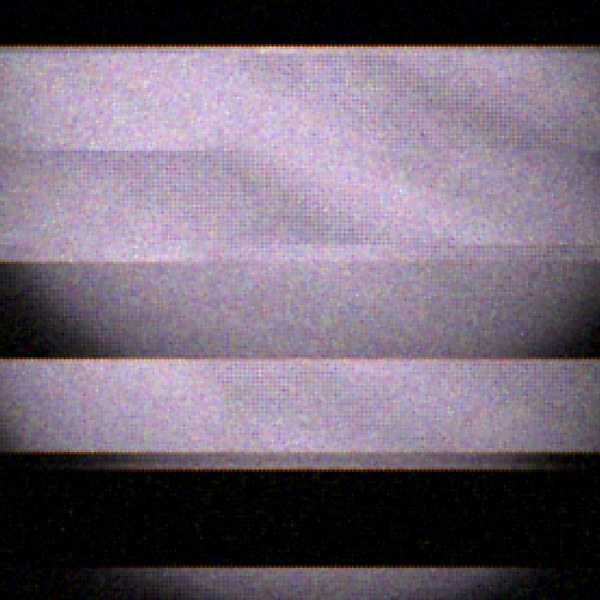
\includegraphics[width=\linewidth]{figures/frame_broken}\\[-1pt]
    {\scriptsize 点数がいちばん高かった「フレーム」}
  \end{minipage}\hfill
  \begin{minipage}[t]{0.36\linewidth}\vspace{0pt}
    この動画には、縞状に乱れた\textbf{壊れたフレーム}が約30枚まじっています。壊れたフレームは模様が異常にくっきりして見えるため、
    品質の点数が飛び抜けて高くなり、時系列のグラフでは \badge{1} のように針のように飛び出します。

    \smallskip
    心配はいりません。\textbf{次のアライメントで、お手本と似ていないフレームとして自動で除外}され（除外した枚数は警告の帯に出ます）、
    グラフも見やすくなります。
  \end{minipage}
\end{caution}

\subsection*{グラフの読み方}

アライメントのあと（壊れたフレームが除外されたあと）の品質グラフは、次のようになります。表示を切り替えると、別のことが分かります。

\noindent
\begin{minipage}[t]{0.47\linewidth}\centering
  \shot[0.62\linewidth]{graph_order}{\mk[e]{cutline}{1}\mk[ne]{best}{2}\mk[nw]{worst}{3}}
  \captionof{figure}{品質順}\label{fig:graph-order}
\end{minipage}\hfill
\begin{minipage}[t]{0.47\linewidth}\centering
  \shot[0.62\linewidth]{graph_timeline}{\mk[e]{cutline}{1}\mk[n]{mode}{4}}
  \captionof{figure}{時系列}\label{fig:graph-timeline}
\end{minipage}

\begin{marklist}
  \item オレンジの線より上のフレームが、参照画像（お手本）の材料になります。
  \item 品質順の左端：いちばん写りのよいフレーム群です。
  \item 右端：写りの悪いフレームです。除外したフレームは、いちばん右にまとめて並びます。
  \item 時系列にすると、撮影中に品質がどう変わったかが分かります。途中で大きく落ちている所があれば、雲が通ったり、ピントがずれたりした可能性があります。
\end{marklist}

グラフをクリックすると、その位置のフレームがプレビューに出ます（緑の縦線が表示中のフレーム）。
採用されたフレームのうち、最良と最悪のものを並べると次のようになります。

\noindent
\begin{minipage}[t]{0.47\linewidth}\centering
  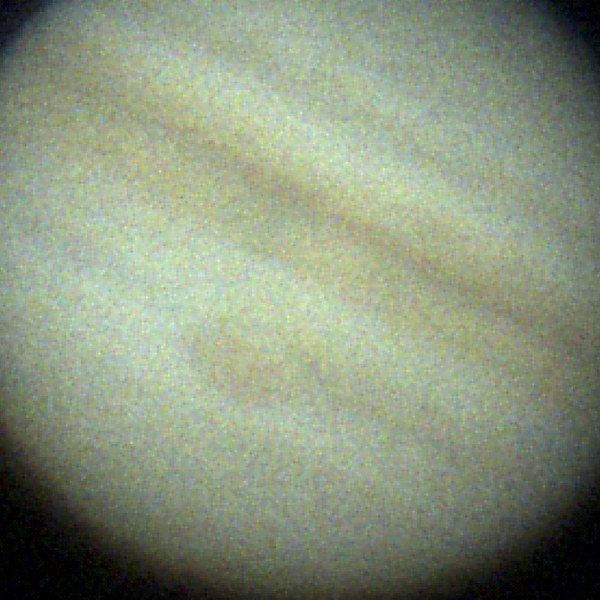
\includegraphics[width=0.8\linewidth]{figures/frame_best}
  \captionof{figure}{品質がいちばん高いフレーム}
\end{minipage}\hfill
\begin{minipage}[t]{0.47\linewidth}\centering
  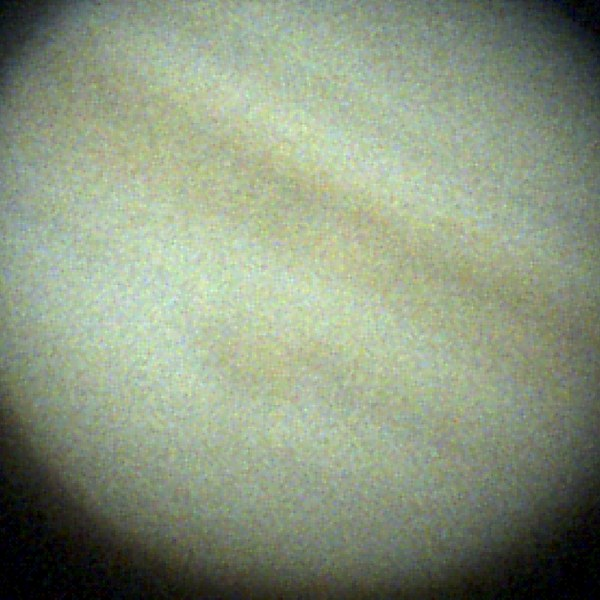
\includegraphics[width=0.8\linewidth]{figures/frame_worst}
  \captionof{figure}{品質がいちばん低いフレーム}
\end{minipage}

\medskip
1枚ずつではどちらもノイズが多く、差は分かりにくいかもしれません。拡大（\uil{200\%}）して縞模様の見え方を比べてみてください。
この「わずかな差」を数千枚ぶん積み重ねるのがスタックです。
% ------------------------------------------------------------------------------
\section{アライメント ——位置を合わせる}\label{sec:qs-align}

\begin{step}{3}{\ui{アライメント} を押す}
  \ui{アライメント} を押します（\key{shift}\key{⌘}\key{A} でも同じ）。次のことを自動で行います。
  \begin{enumerate}[label=(\alph*), itemsep=0pt, topsep=2pt]
    \item 品質の上位25\%のフレームを重ねて、\textbf{参照画像}（お手本）を作る
    \item 惑星の上に\textbf{位置合わせ領域}（四角います目）を自動で並べる
    \item 全フレームについて、ます目ごとに「お手本からどれだけずれているか」と「写りのよさ」を測る
  \end{enumerate}
  終わると「スタック」タブに切り替わって止まります。
\end{step}

\screen{qs_align}{アライメントが終わったところ}{%
  \mk[ne]{banner}{1}\mkd[inw]{preview}{2}\mk[s]{ref}{3}\mk[se]{apcount}{4}\mk[w]{tabs}{5}\mk[w]{aptop}{6}\mk[n]{stack}{7}}

\begin{marklist}
  \item 壊れたフレームや、追跡に失敗したフレーム（惑星が画面の外に出た、など）は自動で除外され、ここに枚数が出ます（この例では 30 枚）。\ui{詳細…} で一覧と理由を見られます。
  \item \textbf{参照画像}と、その上に並んだ\textbf{位置合わせ領域}（水色の四角）。模様のある所にだけ置かれ、背景の暗い宇宙には置かれません。
  \item 表示は自動で \uil{参照} に切り替わっています。
  \item 位置合わせ領域の数と大きさ（ここでは 109 個・48 画素）。
  \item 「スタック」タブに切り替わっています。
  \item 位置合わせ領域ごとに、写りのよい上位何\%のフレームを重ねるか（初期値 10\%）。
  \item \ui{スタック} が押せるようになりました。
\end{marklist}

\begin{center}
\begin{tikzpicture}
  \node[inner sep=0] (ap) {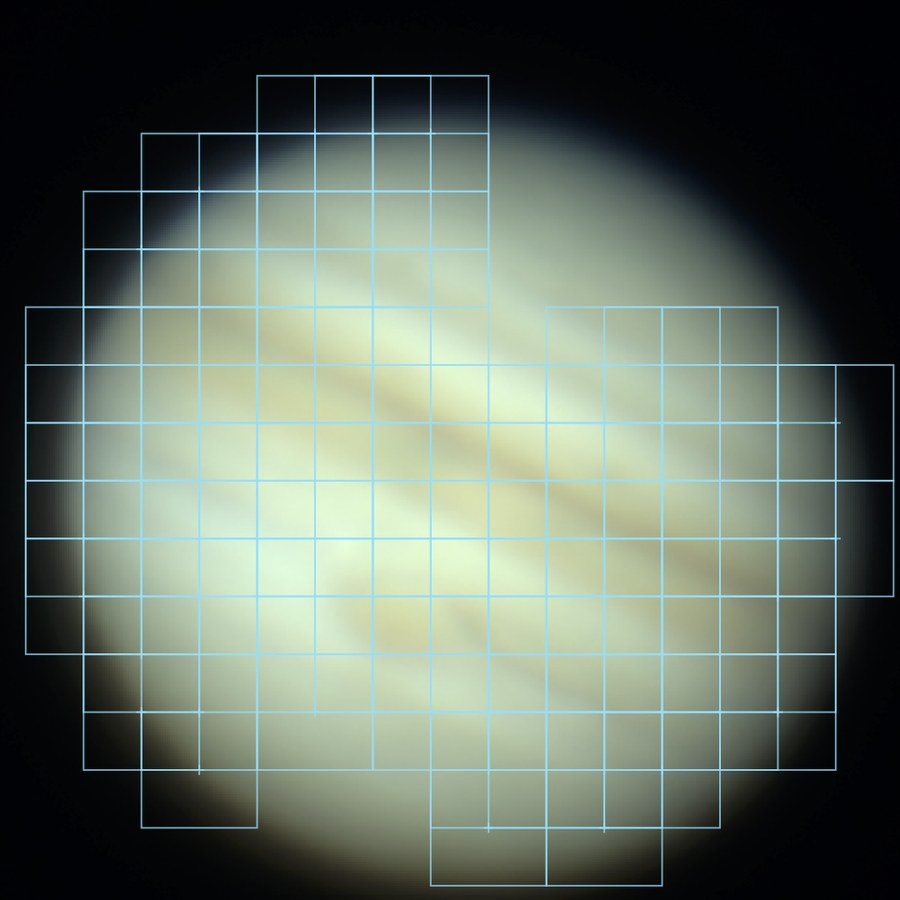
\includegraphics[width=0.5\linewidth]{figures/ap_zoom}};
  \node[lscallout, anchor=west, text width=0.4\linewidth] at ($(ap.east)+(0.5,0.9)$)
    {\small\textbf{なぜ小さな四角に分けるの？}\\[2pt]大気のゆらぎは、場所ごとにずれ方が違います。画像全体を1回で合わせると、
     ある場所は合っても別の場所はずれたままになります。四角ごとに合わせることで、画像全体がくっきりします。
     さらに四角ごとに写りのよいフレームを選ぶので、「このフレームは左上だけよく写っている」という瞬間も生かせます。};
\end{tikzpicture}
\captionof{figure}{参照画像と位置合わせ領域（拡大）}
\end{center}

% ------------------------------------------------------------------------------
\section{スタック ——重ね合わせる}\label{sec:qs-stack}

\begin{step}{4}{\ui{スタック} を押す}
  \ui{スタック} を押します（\key{⌘}\key{R}、またはこのボタンが青いときは \key{return}）。位置合わせ領域ごとに上位10\%のフレームを重ね、
  1枚の画像にまとめます。終わると表示が \uil{結果} に、タブが「仕上げ・出力」に切り替わります。
\end{step}

\screen{qs_stacked}{スタックが終わったところ}{%
  \mkd[inw]{preview}{1}\mk[s]{result}{2}\mk[w]{tabs}{3}\mkd[w]{wavelet}{4}\mk[n]{restack}{5}\mk[n]{export}{6}}

\begin{marklist}
  \item スタックの結果。1枚のフレームと比べて、ざらつきが大きく減っています。ただし、まだ少しぼんやりしています。
        これを次の「仕上げ」でくっきりさせます。
  \item 表示は \uil{結果} になっています。\uil{フレーム} や \uil{参照} に戻して見比べることもできます。
  \item 「仕上げ・出力」タブ。
  \item ウェーブレットなどの仕上げの設定。
  \item 採用率などを変えたら \ui{再スタック}。\textbf{品質評価とアライメントはやり直さない}ので、数秒で終わります。
  \item \ui{書き出し…} が押せるようになりました。
\end{marklist}

\begin{tip}[採用率を変えて試す]
  スタックタブの「位置合わせ領域ごとに採用するフレーム（\%）」を変えて \ui{再スタック} すると、すぐに結果を比べられます。
  上位の割合を減らすと、よい瞬間だけを使うのでシャープになりますが、重ねる枚数が減るのでノイズは増えます。
  目安は第\ref{sec:setting-aptop}節を見てください。
\end{tip}

% ------------------------------------------------------------------------------
\section{仕上げ ——細部を引き出す}\label{sec:qs-finish}

\begin{step}{5}{「仕上げ・出力」タブで調整する}
  仕上げは、スタックの結果を書き換えずに、見え方だけを調整します（何度でもやり直せます）。
  つまみを動かすと、プレビューがすぐに変わります。惑星なら、次の順に進めるのがおすすめです。
  \begin{enumerate}[label=(\alph*), itemsep=1pt, topsep=2pt]
    \item \textbf{RGB チャンネル合わせ}の \ui{自動で合わせる}：縁の赤・青のにじみを取ります。
    \item \textbf{ウェーブレット}：Layer 1〜3 の\uil{強調}を上げて細部を出し、\uil{ノイズ}でざらつきを抑えます。
    \item \textbf{色}の \ui{自動（灰色仮説）}：色かぶりを取ります。必要なら\uil{彩度}を少し上げます。
    \item \textbf{明るさ（レベル補正）}：黒と白の範囲を整えます。
  \end{enumerate}
\end{step}

この例では、次の値にしました（数値の決め方は第\ref{chap:finish}章）。

\begin{center}\small
\begin{tabular}{@{}lcccccc@{}}
\toprule
 & Layer 1 & Layer 2 & Layer 3 & Layer 4 & Layer 5 & Layer 6\\
\midrule
強調 & 12.00 & 7.00 & 3.00 & 1.50 & 1.00 & 1.00\\
ノイズ & 0.45 & 0.25 & 0.05 & 0.00 & 0.00 & 0.00\\
\bottomrule
\end{tabular}
\quad RGB 合わせ・色は \ui{自動}
\end{center}

\noindent
\begin{minipage}[t]{0.32\linewidth}\centering
  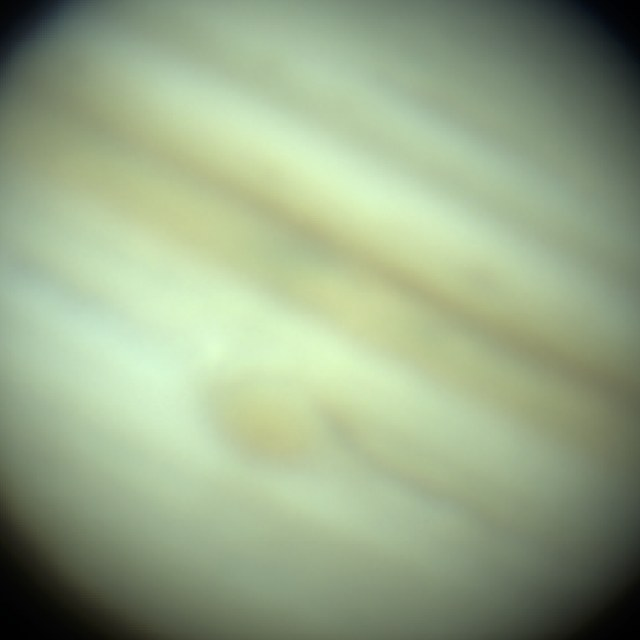
\includegraphics[width=\linewidth]{figures/before_stack}
  \captionof{figure}{スタックしただけ}
\end{minipage}\hfill
\begin{minipage}[t]{0.32\linewidth}\centering
  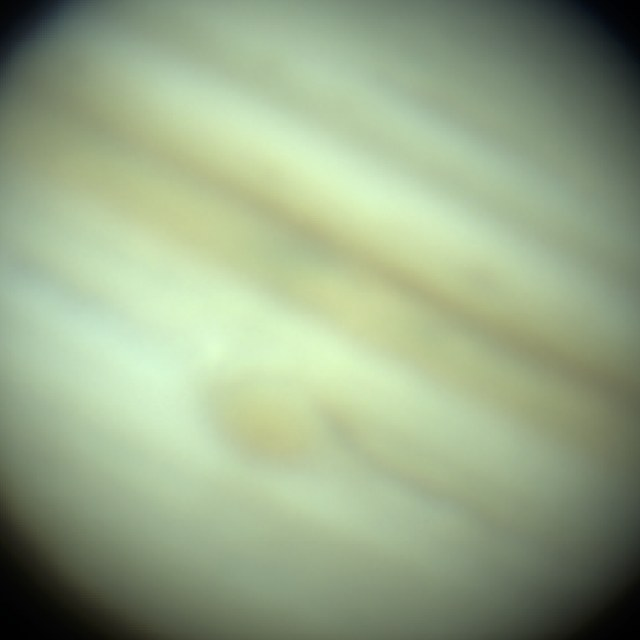
\includegraphics[width=\linewidth]{figures/after_nowave}
  \captionof{figure}{RGB 合わせと色だけ}
\end{minipage}\hfill
\begin{minipage}[t]{0.32\linewidth}\centering
  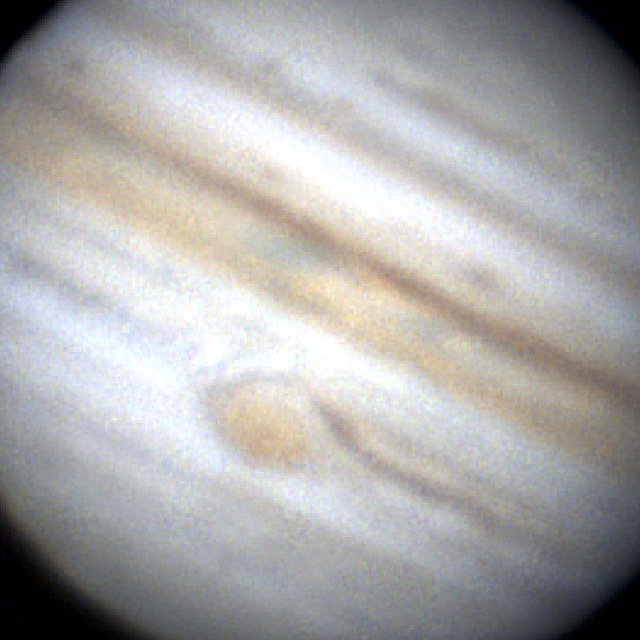
\includegraphics[width=\linewidth]{figures/after_finish}
  \captionof{figure}{ウェーブレットまで}
\end{minipage}

\medskip
ウェーブレットで、縞模様や大赤斑の細部がはっきり見えるようになりました。
強調しすぎるとノイズやふちの不自然な輪（リンギング）が目立つので、プレビューを拡大して確かめながら調整します。

\begin{tip}[効果あり・なしを見比べる]
  「仕上げ・出力」タブのいちばん上の \uil{仕上げ全体の効果をプレビュー} をオフにすると、スタックそのままの画像が出ます。
  ウェーブレット欄の \uil{ウェーブレットの効果をプレビュー} をオフにすると、ウェーブレットだけを外した画像が出ます。
  どちらも\textbf{表示の比較だけ}で、書き出すファイルには設定中の仕上げがすべて入ります。
\end{tip}

% ------------------------------------------------------------------------------
\section{書き出し ——ファイルに保存する}\label{sec:qs-export}

\begin{step}{6}{\ui{書き出し…} を押す}
  「仕上げ・出力」タブのいちばん下の「書き出し」欄で形式を選び、\ui{名前を付けて書き出し…}（または画面下の \ui{書き出し…}、\key{⌘}\key{S}）
  を押します。保存先を選ぶ画面が出るので、場所を決めて保存します。
\end{step}

\sidebyside[0.44]{qs_export}{%
  \mk[w]{format}{1}\mk[w]{name}{2}\mk[w]{object}{3}\mk[w]{meta}{4}\mk[w]{filename}{5}\mk[w]{save}{6}\mk[w]{multi}{7}}{%
  \begin{marklist}
    \item \textbf{形式}：ふつうは \uil{16bit TIFF}。PixInsight などで後処理を続けるなら \uil{32bit float FITS} が便利です。
    \item \textbf{ファイル名の付け方}：\uil{元の名前＋処理条件}、または WinJUPOS で使う \uil{WinJUPOS形式（撮影時刻を先頭に）}。
    \item \textbf{対象名}：「Jupiter」のように入れると、ファイル名と記録に入ります。
    \item 処理条件と撮影時刻をファイルの中に記録します。
    \item 付けられるファイル名の見本（例：\texttt{jupiter\_ap48\_10pct.tif}＝位置合わせ領域 48 画素・採用 10\%）。
    \item 保存します。
    \item 採用率を変えた結果をまとめて保存します（第\ref{sec:multiexport}節）。
  \end{marklist}}

\begin{point}[おつかれさまでした]
  これで一通りの処理ができました。同じファイルを次に開いたときは、保存されたサイドカーから解析結果を読み込むので、
  \ui{スタック} から始められます。次の章からは、各タブの設定をくわしく説明します。
\end{point}
